\chapter{Seeing What We Are}

This chapter follows J. Krishnamurti's first Brockwood Park dialogue in \emph{The Transformation of Man}, curated here for the \emph{How You Got Happiness?} course by LazyingArt LLC through Video2Book. There are no validated blackboard images or equations for this lecture, so the mathematical form used below is deliberately modest: arrows, loops, and tables are editorial reading aids for the spoken inquiry, not a formal system imposed on it. The central movement is from second-hand living to wholeness, from wholeness back to fragmentation, and from fragmentation toward the question of security in knowledge, identity, and the ``me.''

\section{From Second-Hand Life To Wholeness}

The dialogue begins without a prepared thesis. The first question is simply what the three of them should talk about. The proposed theme is that life comes first, not thought or work, and that we ordinarily live through something already made: second-hand words, second-hand roles, second-hand conclusions. This is not yet a doctrine. It is a pressure in the conversation.

Almost immediately the question of wholeness appears. If life is second-hand, fragmented, and lived through inherited structures, then the missing thing seems to be wholeness. But Krishnamurti's first move is to prevent wholeness from becoming a word that consoles us. We cannot begin by saying what the whole is. We begin with what is directly available: the fact that human beings are broken up.

A compact way to mark the opening movement is:

\begin{equation}
\text{second-hand life}
\longrightarrow
\text{question of wholeness}
\longrightarrow
\text{fact of fragmentation}.
\end{equation}

The order matters. Wholeness is not introduced as a metaphysical prize. It is raised because ordinary life is felt to be divided; then it is immediately disciplined by the question of whether we are actually examining ourselves, or merely talking theoretically.

\subsection{Question \& Answer}

\paragraph{Question.}
Can we speak of wholeness while we are fragmented?

\paragraph{Answer.}
Only with great caution. The lecture refuses the quick answer that if we see fragmentation, wholeness is already there. That would be too fast. It would make wholeness into an assumption. The question must be approached from ourselves as we are: fragmented, partial, caught in patches of awareness. The whole may be a meaningful word, but the inquiry has vitality only when it begins with the fragment.

\section{Fragments, Examiner, And Center}

The next problem is not merely that there are fragments. It is whether we can see them. Are we aware of the whole movement of fragmentation, or only of one fragment at a time? Do we see the fragments socially, morally, ethically, religiously, professionally, aesthetically? Or do we take one fragment, examine it, and then assume that examination is enough?

The more severe question is: who is the examiner? If one fragment examines another, the examiner may itself have assumed authority. The observer may be part of the same field it claims to inspect.

Let \(F\) denote the field of fragments and \(Z\) the center that claims to observe or organize them. The lecture does not give this notation; it is only a small map of the spoken movement. The danger is:

\begin{equation}
Z \in F,
\qquad
Z \text{ claims authority over } F.
\end{equation}

That is the trap. The center appears to stand apart, but it is itself a fragment. It seems to be the center of everything because it is in contact with many things: my body, my thoughts, my relations, my pleasures, my fears. But contact is not wholeness. The center is the dominant fragment.

\begin{figure}
\centering
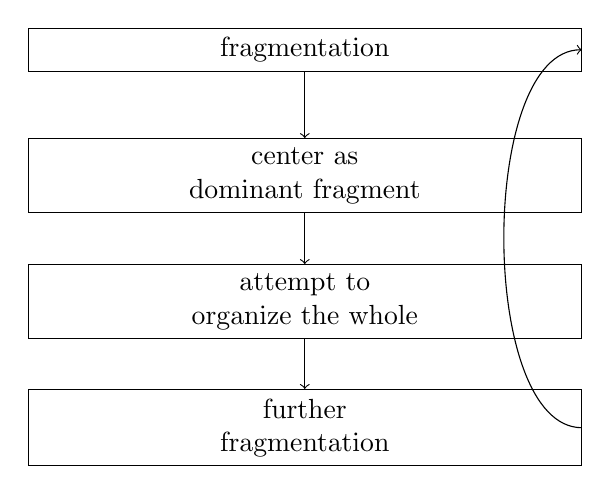
\begin{tikzpicture}
\node[draw, text width=.56\linewidth, align=center] (f) at (0,0) {fragmentation};
\node[draw, text width=.56\linewidth, align=center] (z) at (0,-1.6) {center as\\dominant fragment};
\node[draw, text width=.56\linewidth, align=center] (o) at (0,-3.2) {attempt to\\organize the whole};
\node[draw, text width=.56\linewidth, align=center] (m) at (0,-4.8) {further\\fragmentation};
\draw[->] (f) -- (z);
\draw[->] (z) -- (o);
\draw[->] (o) -- (m);
\draw[->] (m.east) .. controls (2.2,-4.8) and (2.2,0) .. (f.east);
\end{tikzpicture}
\caption{An editorial reconstruction of the loop developed in the dialogue: fragmentation breeds the center, and the center sustains further fragmentation. No original board diagram was available.}
\end{figure}

\section{Conflict As The Usual Door To Awareness}

The lecture then asks a sharper question: when are we actually aware of fragmentation? The answer developed in the dialogue is not flattering. We usually become aware only when there is contradiction, and contradiction becomes conflict. The pain or unpleasantness of conflict makes us say that something is wrong.

The useful schematic is:

\begin{equation}
\text{fragmentation}
\longrightarrow
\text{contradiction}
\longrightarrow
\text{conflict}
\longrightarrow
\text{self-conscious awareness}.
\end{equation}

This is not a psychological law. It is a reading map of the conversation. Opposing desires, wishes, thoughts, and identities collide; the collision produces conflict; conflict produces the sense, ``I am in conflict.'' Without pain or intense pleasure, we may not be aware of ourselves at all.

\subsection{Question \& Answer}

\paragraph{Question.}
Are we aware of fragmentation itself, or only of conflict?

\paragraph{Answer.}
Ordinarily, only of conflict. The lecture says that where there is conflict, there is awareness of contradiction. Fragmentation with its conflict brings the sense of ``I am aware'' or ``I am in conflict.'' This leaves open a later and deeper question: whether there can be awareness without conflict. In this lecture that different approach is named, but not yet unfolded.

\paragraph{A worked chain.}
Take two identities or desires, \(A\) and \(B\), each claiming importance.

\begin{align}
A & = \text{a fragment treated as decisive}, \\
B & = \text{another fragment treated as decisive}, \\
A \perp B & \longrightarrow \text{contradiction}, \\
\text{contradiction} & \longrightarrow \text{conflict}, \\
\text{conflict} & \longrightarrow \text{awareness of fragmentation}.
\end{align}

The symbol \(\perp\) here means opposition, not a technical orthogonality. It is a compact way of preserving the lecture's repeated point: we usually discover division because the divisions hurt.

\section{The Fragment Claims To Be The Whole}

The inquiry then moves from inner structure to concrete examples. A person says, ``I am a Hindu,'' ``I am a Jew,'' ``I am an Arab,'' ``I am a communist,'' ``I am a Catholic,'' ``I am a businessman,'' ``I am an artist,'' ``I am a scientist,'' or ``I am a doctor.'' These are not neutral descriptions when they become psychologically total. The trouble begins when the part claims the whole person.

The editorial shorthand is:

\begin{equation}
\text{part} \;\widehat{=}\; \text{whole}.
\end{equation}

The symbol \(\widehat{=}\) means ``is taken as,'' not actual equality. The fragment does not become the whole; it is treated as though it were the whole. Then another person or group does the same with a different fragment. One totalized part faces another totalized part, and conflict becomes almost inevitable.

\begin{proposition}
When a fragment is treated as the whole of the person, it becomes structurally conflict-producing.
\end{proposition}

\begin{proof}
A fragment can function in its place. A professional skill, a language, a task, or a practical role may be limited and useful. Conflict enters when the fragment says, implicitly or explicitly, ``I am the whole.'' Then another fragment makes the same claim. Since both cannot occupy the whole without contradiction, the relation becomes oppositional. The proof is not formal psychology; it is the structure of the examples in the dialogue.
\end{proof}

This is why the social examples are not decorative. Northern Ireland, the Middle East, religious divisions, political divisions, professional prestige, and the doctor protected by the medical community all illustrate the same movement: a partial structure claims total significance.

\section{What Causes Fragmentation?}

At the midpoint the lecture turns from description to cause. Several quick answers are tried and refused. Is fear the cause? Krishnamurti presses further: perhaps fragmentation causes fear. Is it childhood separation, holding on, the mother and child, biological separation? Again the answer is slowed down. The inquiry is not looking for a remote historical or genetic origin. It asks what action sustains fragmentation now.

The first causal map is therefore cautious:

\begin{equation}
\text{fragmentation}
\longrightarrow
\text{fear}
\qquad
\text{rather than simply}
\qquad
\text{fear}
\longrightarrow
\text{fragmentation}.
\end{equation}

The correction is important. Fear is present, but the lecture does not let fear become the easy explanatory master-word. The question is: what is the movement that makes one say, ``I am this,'' and then live inside that enclosure?

\subsection{Question \& Answer}

\paragraph{Question.}
Is fear the cause of fragmentation, or does fragmentation generate fear?

\paragraph{Answer.}
The dialogue leans toward the second formulation, while keeping the whole matter under inquiry. Fear is not denied, but Krishnamurti resists making it the first cause. Fragmentation creates insecurity; insecurity produces fear; fear then helps preserve the structures that promised security. The movement is circular, but the lecture keeps asking us to look at the present action rather than settle for a theory.

A more useful local update rule is:

\begin{align}
\text{identity} &\longrightarrow \text{belonging}, \\
\text{belonging} &\longrightarrow \text{felt protection}, \\
\text{felt protection} &\longrightarrow \text{dependence}, \\
\text{dependence} &\longrightarrow \text{fear of exclusion}, \\
\text{fear of exclusion} &\longrightarrow \text{stronger identity}.
\end{align}

This is one of the lecture's central loops. The person seeks safety in the fragment, then becomes afraid to question the fragment, because questioning may mean losing the group, the position, the profession, or the name.

\section{Knowledge In Its Right Place}

The inquiry next asks whether knowledge is the source of fragmentation. Again, the answer is not blunt. Knowledge is not condemned. Driving a car, learning a language, carrying out a technical task: these require knowledge. A limited object can be handled by limited knowledge. The difficulty begins when knowledge, which belongs to the past, claims to know the living present as a whole.

\begin{equation}
\text{knowledge of the past}
\;\not=\;
\text{direct perception of the present}.
\end{equation}

To say ``I have known you'' may be accurate in a limited sense. To say ``I know you'' is already dangerous, because the other person is moving, changing, alive. The past is then imposed on the present. The part covers the whole.

\begin{table}
\centering
\begin{tabular}{p{.42\linewidth} p{.42\linewidth}}
\hline
Knowledge in place & Knowledge out of place \\
\hline
Driving a car & ``I know you'' \\
Learning a language & ``I know myself'' \\
Technical action & ``I know the whole of life'' \\
Limited object, limited use & Theory of the whole used for psychological security \\
\hline
\end{tabular}
\caption{A compact reconstruction of the lecture's distinction between practical knowledge and psychological misuse of knowledge.}
\end{table}

We can summarize the distinction as:

\begin{equation}
K_{\mathrm{practical}} \text{ has its place},
\qquad
K_{\psi} \text{ fragments when it claims the whole}.
\end{equation}

Here \(K_{\psi}\) denotes psychological knowledge: knowledge used to define myself, another person, life, status, God, or the universe in order to feel secure. The danger is not knowledge as such, but confusion about its role.

\subsection{Question \& Answer}

\paragraph{Question.}
Why is practical knowledge not fragmentation, while psychological knowledge becomes fragmentary?

\paragraph{Answer.}
Because practical knowledge operates on a limited field. A car, a language lesson, or a technical procedure can be approached as a part. But when the same movement says, ``I know the whole of you,'' or ``I know what I am,'' or ``I know what life is,'' a part of the past is being imposed on a living whole. The lecture's phrase is not anti-knowledge; it is an attempt to put knowledge in its right place.

\section{Psychological Security And The Me}

The final movement brings knowledge and identity into the question of security. Biological security is necessary: food, clothing, shelter, physical protection. But the lecture argues that the search for psychological security in ideas, images, conclusions, groups, status, knowledge, and the ``me'' prevents shared physical security.

The ladder is narrow and severe:

\begin{figure}
\centering
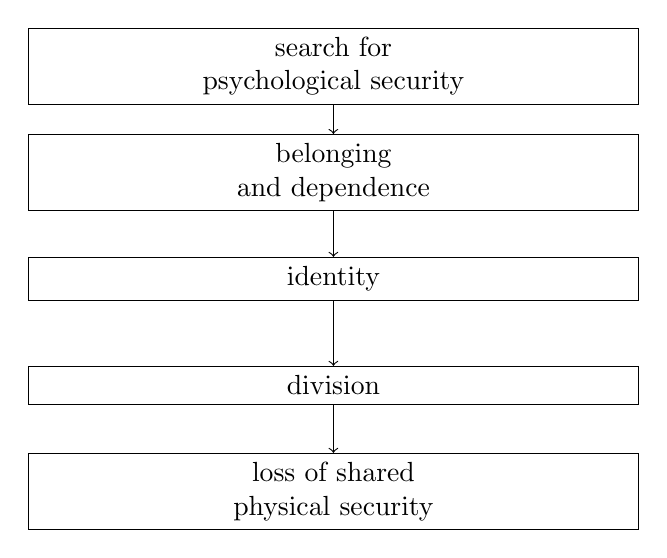
\begin{tikzpicture}
\node[draw, text width=.62\linewidth, align=center] (a) at (0,0) {search for\\psychological security};
\node[draw, text width=.62\linewidth, align=center] (b) at (0,-1.35) {belonging\\and dependence};
\node[draw, text width=.62\linewidth, align=center] (c) at (0,-2.7) {identity};
\node[draw, text width=.62\linewidth, align=center] (d) at (0,-4.05) {division};
\node[draw, text width=.62\linewidth, align=center] (e) at (0,-5.4) {loss of shared\\physical security};
\draw[->] (a) -- (b);
\draw[->] (b) -- (c);
\draw[->] (c) -- (d);
\draw[->] (d) -- (e);
\end{tikzpicture}
\caption{A pocket-size causal ladder reconstructed from the closing movement of the dialogue.}
\end{figure}

In symbols:

\begin{equation}
S_{\psi}(\text{group, image, conclusion, me})
\longrightarrow
\text{fragmentation}
\longrightarrow
\neg S_{\mathrm{bio/shared}}.
\end{equation}

This is the lecture's unsettling reversal. The person thinks psychological security is the route to safety. But the search for psychological security creates divisions that undermine the wider biological security of all: food, shelter, education, and the absence of war.

The last step is the ``me.'' Psychological security gathers around the possessive center: my position, my happiness, my money, my house, my wife, my country, my God. The lecture does not close by resolving this. It closes by naming it as the fact to be faced:

\begin{equation}
\text{me}
\longrightarrow
\text{greatest psychological security}.
\end{equation}

The ``me'' is treated as the essence of the whole. If the me is threatened, the world seems to lose meaning. If the me is important, its country, its God, its status, and its happiness become important. The chapter should stop where the dialogue stops: not with a solution, but with a pressure that points forward.

\section{Summary}

The lecture's movement can be read as a sequence of disciplined refusals. Do not begin with a theory of wholeness. Do not assume the examiner is outside fragmentation. Do not mistake the center for the whole. Do not say fear is the simple cause before looking at the present movement. Do not condemn knowledge, but put it in its place. Do not confuse psychological security with biological security.

The conceptual spine is:

\begin{equation}
\text{fragment}
\longrightarrow
\text{center}
\longrightarrow
\text{conflict}
\longrightarrow
\text{search for security}
\longrightarrow
\text{me}.
\end{equation}

This is an editorial map, not Krishnamurti's notation. The transcript's force lies in the way each term is discovered in conversation. Fragmentation is not an abstract defect; it is the living movement by which a part claims the whole. Knowledge is not rejected; it becomes dangerous when the past claims the present. Security is not dismissed; biological security is necessary, but psychological security in the ``me'' produces division. The next inquiry must begin from that unresolved fact.